% Adapted from https://texample.net/tikz/examples/periodic-table-of-chemical-elements.
% All Credit to Ivan Griffin.

\documentclass[tikz,border=5mm]{standalone}
\usetikzlibrary{shapes,calc}

\begin{document}

\newcommand{\ElemLabel}[4]{
    \begin{minipage}{2.2cm}
        \centering
        {\textbf{#1} \hfill #2}%
        \linebreak \linebreak
        {\textbf{#3}}%
        \linebreak \linebreak
        {{#4}}
    \end{minipage}
}

\newcommand{\NaturalElem}[4]{\ElemLabel{#1}{#2}{\huge {#3}}{#4}}

\newcommand{\SyntheticElem}[4]{\ElemLabel{#1}{#2}{\color{gray}{\huge #3}}{#4}}

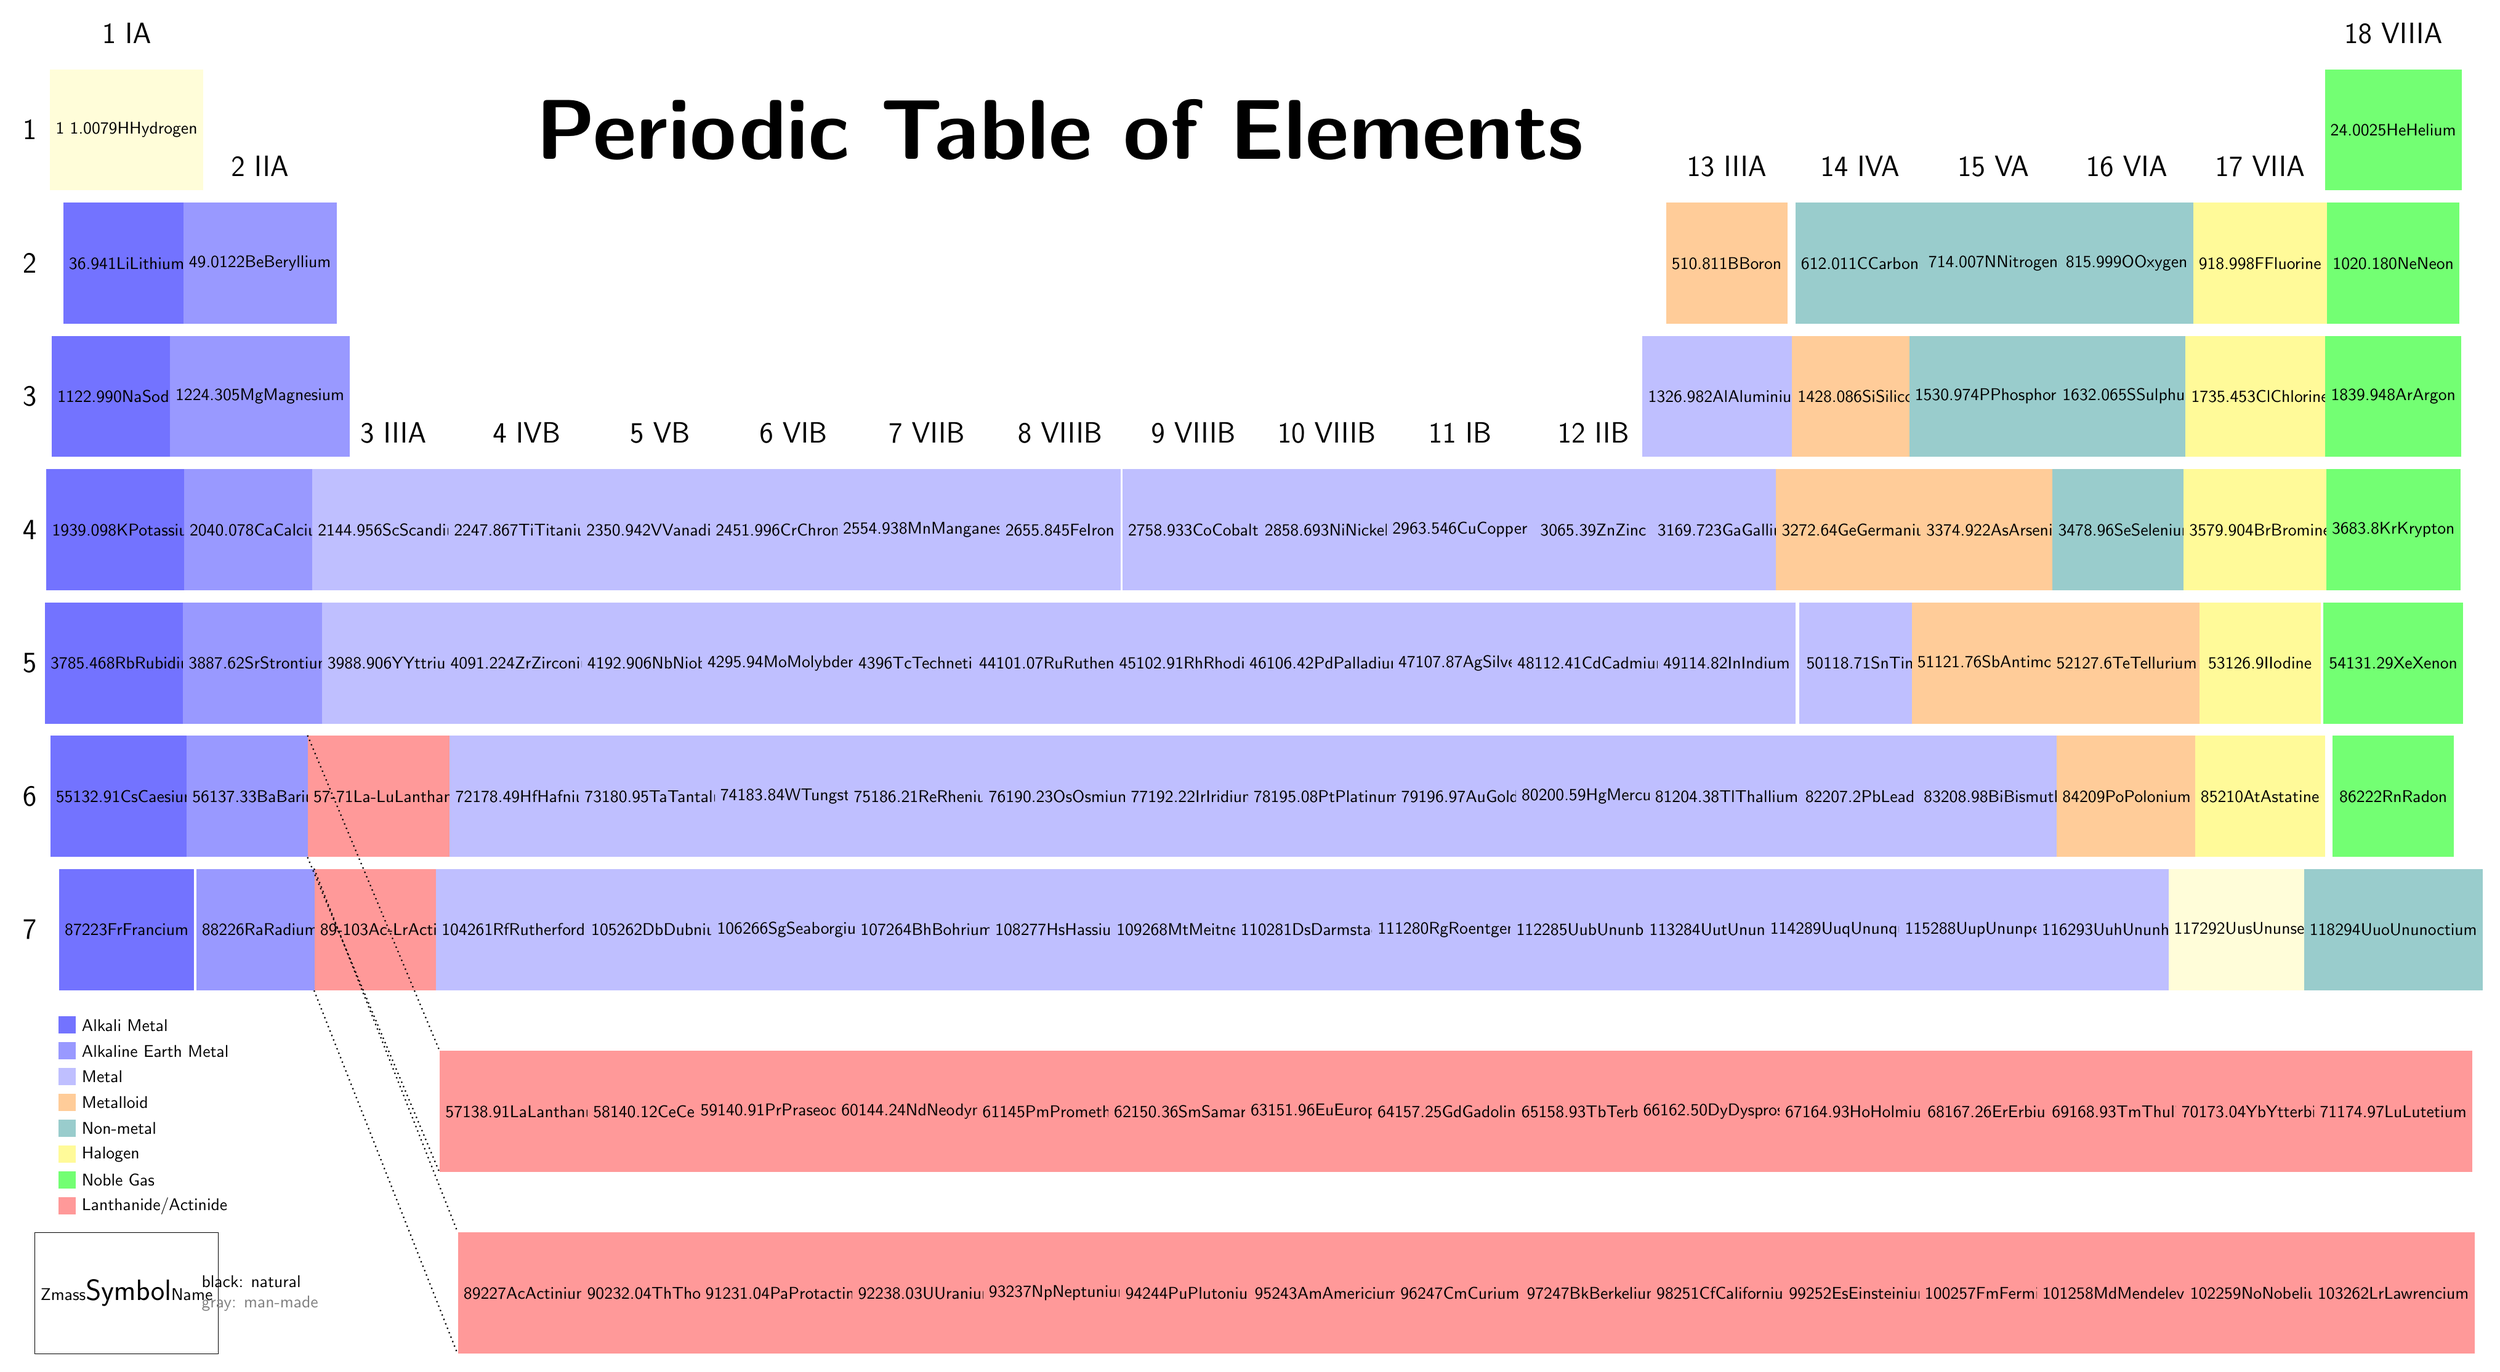
\begin{tikzpicture}[font=\sffamily]

    % Fill Color Styles
    \tikzstyle{ElementFill} = [fill=yellow!15]
    \tikzstyle{AlkaliMetalFill} = [fill=blue!55]
    \tikzstyle{AlkalineEarthMetalFill} = [fill=blue!40]
    \tikzstyle{MetalFill} = [fill=blue!25]
    \tikzstyle{MetalloidFill} = [fill=orange!40]
    \tikzstyle{NonmetalFill} = [fill=teal!40]
    \tikzstyle{HalogenFill} = [fill=yellow!40]
    \tikzstyle{NobleGasFill} = [fill=green!55]
    \tikzstyle{LanthanideActinideFill} = [fill=red!40]

    % Element Styles
    \tikzstyle{Element} = [ElementFill,
    minimum width=2.5cm, minimum height=2.5cm, node distance=2.75cm]
    \tikzstyle{AlkaliMetal} = [Element, AlkaliMetalFill]
    \tikzstyle{AlkalineEarthMetal} = [Element, AlkalineEarthMetalFill]
    \tikzstyle{Metal} = [Element, MetalFill]
    \tikzstyle{Metalloid} = [Element, MetalloidFill]
    \tikzstyle{Nonmetal} = [Element, NonmetalFill]
    \tikzstyle{Halogen} = [Element, HalogenFill]
    \tikzstyle{NobleGas} = [Element, NobleGasFill]
    \tikzstyle{LanthanideActinide} = [Element, LanthanideActinideFill]
    \tikzstyle{PeriodLabel} = [font={\sffamily\LARGE}, node distance=2.0cm]
    \tikzstyle{GroupLabel} = [font={\sffamily\LARGE}, minimum width=2.75cm, node distance=2.0cm]

    % Group 1 - IA
    \node[Element] (H) {\NaturalElem{1} {1.0079}{H}{Hydrogen}};
    \node[below of=H, AlkaliMetal] (Li) {\NaturalElem{3}{6.941}{Li}{Lithium}};
    \node[below of=Li, AlkaliMetal] (Na) {\NaturalElem{11}{22.990}{Na}{Sodium}};
    \node[below of=Na, AlkaliMetal] (K) {\NaturalElem{19}{39.098}{K}{Potassium}};
    \node[below of=K, AlkaliMetal] (Rb) {\NaturalElem{37}{85.468}{Rb}{Rubidium}};
    \node[below of=Rb, AlkaliMetal] (Cs) {\NaturalElem{55}{132.91}{Cs}{Caesium}};
    \node[below of=Cs, AlkaliMetal] (Fr) {\NaturalElem{87}{223}{Fr}{Francium}};

    % Group 2 - IIA
    \node[right of=Li, AlkalineEarthMetal] (Be) {\NaturalElem{4}{9.0122}{Be}{Beryllium}};
    \node[below of=Be, AlkalineEarthMetal] (Mg) {\NaturalElem{12}{24.305}{Mg}{Magnesium}};
    \node[below of=Mg, AlkalineEarthMetal] (Ca) {\NaturalElem{20}{40.078}{Ca}{Calcium}};
    \node[below of=Ca, AlkalineEarthMetal] (Sr) {\NaturalElem{38}{87.62}{Sr}{Strontium}};
    \node[below of=Sr, AlkalineEarthMetal] (Ba) {\NaturalElem{56}{137.33}{Ba}{Barium}};
    \node[below of=Ba, AlkalineEarthMetal] (Ra) {\NaturalElem{88}{226}{Ra}{Radium}};

    % Group 3 - IIIB
    \node[right of=Ca, Metal] (Sc) {\NaturalElem{21}{44.956}{Sc}{Scandium}};
    \node[below of=Sc, Metal] (Y) {\NaturalElem{39}{88.906}{Y}{Yttrium}};
    \node[below of=Y, LanthanideActinide] (LaLu) {\NaturalElem{57-71}{}{La-Lu}{Lanthanide}};
    \node[below of=LaLu, LanthanideActinide] (AcLr) {\NaturalElem{89-103}{}{Ac-Lr}{Actinide}};

    % Group 4 - IVB
    \node[right of=Sc, Metal] (Ti) {\NaturalElem{22}{47.867}{Ti}{Titanium}};
    \node[below of=Ti, Metal] (Zr) {\NaturalElem{40}{91.224}{Zr}{Zirconium}};
    \node[below of=Zr, Metal] (Hf) {\NaturalElem{72}{178.49}{Hf}{Hafnium}};
    \node[below of=Hf, Metal] (Rf) {\SyntheticElem{104}{261}{Rf}{Rutherfordium}};

    % Group 5 - VB
    \node[right of=Ti, Metal] (V) {\NaturalElem{23}{50.942}{V}{Vanadium}};
    \node[below of=V, Metal] (Nb) {\NaturalElem{41}{92.906}{Nb}{Niobium}};
    \node[below of=Nb, Metal] (Ta) {\NaturalElem{73}{180.95}{Ta}{Tantalum}};
    \node[below of=Ta, Metal] (Db) {\SyntheticElem{105}{262}{Db}{Dubnium}};

    % Group 6 - VIB
    \node[right of=V, Metal] (Cr) {\NaturalElem{24}{51.996}{Cr}{Chromium}};
    \node[below of=Cr, Metal] (Mo) {\NaturalElem{42}{95.94}{Mo}{Molybdenum}};
    \node[below of=Mo, Metal] (W) {\NaturalElem{74}{183.84}{W}{Tungsten}};
    \node[below of=W, Metal] (Sg) {\SyntheticElem{106}{266}{Sg}{Seaborgium}};

    % Group 7 - VIIB
    \node[right of=Cr, Metal] (Mn) {\NaturalElem{25}{54.938}{Mn}{Manganese}};
    \node[below of=Mn, Metal] (Tc) {\NaturalElem{43}{96}{Tc}{Technetium}};
    \node[below of=Tc, Metal] (Re) {\NaturalElem{75}{186.21}{Re}{Rhenium}};
    \node[below of=Re, Metal] (Bh) {\SyntheticElem{107}{264}{Bh}{Bohrium}};

    % Group 8 - VIIIB
    \node[right of=Mn, Metal] (Fe) {\NaturalElem{26}{55.845}{Fe}{Iron}};
    \node[below of=Fe, Metal] (Ru) {\NaturalElem{44}{101.07}{Ru}{Ruthenium}};
    \node[below of=Ru, Metal] (Os) {\NaturalElem{76}{190.23}{Os}{Osmium}};
    \node[below of=Os, Metal] (Hs) {\SyntheticElem{108}{277}{Hs}{Hassium}};

    % Group 9 - VIIIB
    \node[right of=Fe, Metal] (Co) {\NaturalElem{27}{58.933}{Co}{Cobalt}};
    \node[below of=Co, Metal] (Rh) {\NaturalElem{45}{102.91}{Rh}{Rhodium}};
    \node[below of=Rh, Metal] (Ir) {\NaturalElem{77}{192.22}{Ir}{Iridium}};
    \node[below of=Ir, Metal] (Mt) {\SyntheticElem{109}{268}{Mt}{Meitnerium}};

    % Group 10 - VIIIB
    \node[right of=Co, Metal] (Ni) {\NaturalElem{28}{58.693}{Ni}{Nickel}};
    \node[below of=Ni, Metal] (Pd) {\NaturalElem{46}{106.42}{Pd}{Palladium}};
    \node[below of=Pd, Metal] (Pt) {\NaturalElem{78}{195.08}{Pt}{Platinum}};
    \node[below of=Pt, Metal] (Ds) {\SyntheticElem{110}{281}{Ds}{Darmstadtium}};

    % Group 11 - IB
    \node[right of=Ni, Metal] (Cu) {\NaturalElem{29}{63.546}{Cu}{Copper}};
    \node[below of=Cu, Metal] (Ag) {\NaturalElem{47}{107.87}{Ag}{Silver}};
    \node[below of=Ag, Metal] (Au) {\NaturalElem{79}{196.97}{Au}{Gold}};
    \node[below of=Au, Metal] (Rg) {\SyntheticElem{111}{280}{Rg}{Roentgenium}};

    % Group 12 - IIB
    \node[right of=Cu, Metal] (Zn) {\NaturalElem{30}{65.39}{Zn}{Zinc}};
    \node[below of=Zn, Metal] (Cd) {\NaturalElem{48}{112.41}{Cd}{Cadmium}};
    \node[below of=Cd, Metal] (Hg) {\NaturalElem{80}{200.59}{Hg}{Mercury}};
    \node[below of=Hg, Metal] (Uub) {\SyntheticElem{112}{285}{Uub}{Ununbium}};

    % Group 13 - IIIA
    \node[right of=Zn, Metal] (Ga) {\NaturalElem{31}{69.723}{Ga}{Gallium}};
    \node[above of=Ga, Metal] (Al) {\NaturalElem{13}{26.982}{Al}{Aluminium}};
    \node[above of=Al, Metalloid] (B) {\NaturalElem{5}{10.811}{B}{Boron}};
    \node[below of=Ga, Metal] (In) {\NaturalElem{49}{114.82}{In}{Indium}};
    \node[below of=In, Metal] (Tl) {\NaturalElem{81}{204.38}{Tl}{Thallium}};
    \node[below of=Tl, Metal] (Uut) {\SyntheticElem{113}{284}{Uut}{Ununtrium}};

    % Group 14 - IVA
    \node[right of=B, Nonmetal] (C) {\NaturalElem{6}{12.011}{C}{Carbon}};
    \node[below of=C, Metalloid] (Si) {\NaturalElem{14}{28.086}{Si}{Silicon}};
    \node[below of=Si, Metalloid] (Ge) {\NaturalElem{32}{72.64}{Ge}{Germanium}};
    \node[below of=Ge, Metal] (Sn) {\NaturalElem{50}{118.71}{Sn}{Tin}};
    \node[below of=Sn, Metal] (Pb) {\NaturalElem{82}{207.2}{Pb}{Lead}};
    \node[below of=Pb, Metal] (Uuq) {\SyntheticElem{114}{289}{Uuq}{Ununquadium}};

    % Group 15 - VA
    \node[right of=C, Nonmetal] (N) {\NaturalElem{7}{14.007}{N}{Nitrogen}};
    \node[below of=N, Nonmetal] (P) {\NaturalElem{15}{30.974}{P}{Phosphorus}};
    \node[below of=P, Metalloid] (As) {\NaturalElem{33}{74.922}{As}{Arsenic}};
    \node[below of=As, Metalloid] (Sb) {\NaturalElem{51}{121.76}{Sb}{Antimony}};
    \node[below of=Sb, Metal] (Bi) {\NaturalElem{83}{208.98}{Bi}{Bismuth}};
    \node[below of=Bi, Metal] (Uup) {\SyntheticElem{115}{288}{Uup}{Ununpentium}};

    % Group 16 - VIA
    \node[right of=N, Nonmetal] (O) {\NaturalElem{8}{15.999}{O}{Oxygen}};
    \node[below of=O, Nonmetal] (S) {\NaturalElem{16}{32.065}{S}{Sulphur}};
    \node[below of=S, Nonmetal] (Se) {\NaturalElem{34}{78.96}{Se}{Selenium}};
    \node[below of=Se, Metalloid] (Te) {\NaturalElem{52}{127.6}{Te}{Tellurium}};
    \node[below of=Te, Metalloid] (Po) {\NaturalElem{84}{209}{Po}{Polonium}};
    \node[below of=Po, Metal] (Uuh) {\SyntheticElem{116}{293}{Uuh}{Ununhexium}};

    % Group 17 - VIIA
    \node[right of=O, Halogen] (F) {\NaturalElem{9}{18.998}{F}{Fluorine}};
    \node[below of=F, Halogen] (Cl) {\NaturalElem{17}{35.453}{Cl}{Chlorine}};
    \node[below of=Cl, Halogen] (Br) {\NaturalElem{35}{79.904}{Br}{Bromine}};
    \node[below of=Br, Halogen] (I) {\NaturalElem{53}{126.9}{I}{Iodine}};
    \node[below of=I, Halogen] (At) {\NaturalElem{85}{210}{At}{Astatine}};
    \node[below of=At, Element] (Uus) {\SyntheticElem{117}{292}{Uus}{Ununseptium}};

    % Group 18 - VIIIA
    \node[right of=F, NobleGas] (Ne) {\NaturalElem{10}{20.180}{Ne}{Neon}};
    \node[above of=Ne, NobleGas] (He) {\NaturalElem{2}{4.0025}{He}{Helium}};
    \node[below of=Ne, NobleGas] (Ar) {\NaturalElem{18}{39.948}{Ar}{Argon}};
    \node[below of=Ar, NobleGas] (Kr) {\NaturalElem{36}{83.8}{Kr}{Krypton}};
    \node[below of=Kr, NobleGas] (Xe) {\NaturalElem{54}{131.29}{Xe}{Xenon}};
    \node[below of=Xe, NobleGas] (Rn) {\NaturalElem{86}{222}{Rn}{Radon}};
    \node[below of=Rn, Nonmetal] (Uuo) {\SyntheticElem{118}{294}{Uuo}{Ununoctium}};

    % Period
    \node[left of=H, PeriodLabel] (Period1) {1};
    \node[left of=Li, PeriodLabel] (Period2) {2};
    \node[left of=Na, PeriodLabel] (Period3) {3};
    \node[left of=K, PeriodLabel] (Period4) {4};
    \node[left of=Rb, PeriodLabel] (Period5) {5};
    \node[left of=Cs, PeriodLabel] (Period6) {6};
    \node[left of=Fr, PeriodLabel] (Period7) {7};

    % Group
    \node[above of=H, GroupLabel] (Group1) {1 \hfill IA};
    \node[above of=Be, GroupLabel] (Group2) {2 \hfill IIA};
    \node[above of=Sc, GroupLabel] (Group3) {3 \hfill IIIA};
    \node[above of=Ti, GroupLabel] (Group4) {4 \hfill IVB};
    \node[above of=V, GroupLabel] (Group5) {5 \hfill VB};
    \node[above of=Cr, GroupLabel] (Group6) {6 \hfill VIB};
    \node[above of=Mn, GroupLabel] (Group7) {7 \hfill VIIB};
    \node[above of=Fe, GroupLabel] (Group8) {8 \hfill VIIIB};
    \node[above of=Co, GroupLabel] (Group9) {9 \hfill VIIIB};
    \node[above of=Ni, GroupLabel] (Group10) {10 \hfill VIIIB};
    \node[above of=Cu, GroupLabel] (Group11) {11 \hfill IB};
    \node[above of=Zn, GroupLabel] (Group12) {12 \hfill IIB};
    \node[above of=B, GroupLabel] (Group13) {13 \hfill IIIA};
    \node[above of=C, GroupLabel] (Group14) {14 \hfill IVA};
    \node[above of=N, GroupLabel] (Group15) {15 \hfill VA};
    \node[above of=O, GroupLabel] (Group16) {16 \hfill VIA};
    \node[above of=F, GroupLabel] (Group17) {17 \hfill VIIA};
    \node[above of=He, GroupLabel] (Group18) {18 \hfill VIIIA};

    % Lanthanide
    \node[below of=Rf, LanthanideActinide, yshift=-1cm] (La) {\NaturalElem{57}{138.91}{La}{Lanthanum}};
    \node[right of=La, LanthanideActinide] (Ce) {\NaturalElem{58}{140.12}{Ce}{Cerium}};
    \node[right of=Ce, LanthanideActinide] (Pr) {\NaturalElem{59}{140.91}{Pr}{Praseodymium}};
    \node[right of=Pr, LanthanideActinide] (Nd) {\NaturalElem{60}{144.24}{Nd}{Neodymium}};
    \node[right of=Nd, LanthanideActinide] (Pm) {\NaturalElem{61}{145}{Pm}{Promethium}};
    \node[right of=Pm, LanthanideActinide] (Sm) {\NaturalElem{62}{150.36}{Sm}{Samarium}};
    \node[right of=Sm, LanthanideActinide] (Eu) {\NaturalElem{63}{151.96}{Eu}{Europium}};
    \node[right of=Eu, LanthanideActinide] (Gd) {\NaturalElem{64}{157.25}{Gd}{Gadolinium}};
    \node[right of=Gd, LanthanideActinide] (Tb) {\NaturalElem{65}{158.93}{Tb}{Terbium}};
    \node[right of=Tb, LanthanideActinide] (Dy) {\NaturalElem{66}{162.50}{Dy}{Dysprosium}};
    \node[right of=Dy, LanthanideActinide] (Ho) {\NaturalElem{67}{164.93}{Ho}{Holmium}};
    \node[right of=Ho, LanthanideActinide] (Er) {\NaturalElem{68}{167.26}{Er}{Erbium}};
    \node[right of=Er, LanthanideActinide] (Tm) {\NaturalElem{69}{168.93}{Tm}{Thulium}};
    \node[right of=Tm, LanthanideActinide] (Yb) {\NaturalElem{70}{173.04}{Yb}{Ytterbium}};
    \node[right of=Yb, LanthanideActinide] (Lu) {\NaturalElem{71}{174.97}{Lu}{Lutetium}};

    % Actinide
    \node[below of=La, LanthanideActinide, yshift=-1cm] (Ac) {\NaturalElem{89}{227}{Ac}{Actinium}};
    \node[right of=Ac, LanthanideActinide] (Th) {\NaturalElem{90}{232.04}{Th}{Thorium}};
    \node[right of=Th, LanthanideActinide] (Pa) {\NaturalElem{91}{231.04}{Pa}{Protactinium}};
    \node[right of=Pa, LanthanideActinide] (U) {\NaturalElem{92}{238.03}{U}{Uranium}};
    \node[right of=U, LanthanideActinide] (Np) {\SyntheticElem{93}{237}{Np}{Neptunium}};
    \node[right of=Np, LanthanideActinide] (Pu) {\SyntheticElem{94}{244}{Pu}{Plutonium}};
    \node[right of=Pu, LanthanideActinide] (Am) {\SyntheticElem{95}{243}{Am}{Americium}};
    \node[right of=Am, LanthanideActinide] (Cm) {\SyntheticElem{96}{247}{Cm}{Curium}};
    \node[right of=Cm, LanthanideActinide] (Bk) {\SyntheticElem{97}{247}{Bk}{Berkelium}};
    \node[right of=Bk, LanthanideActinide] (Cf) {\SyntheticElem{98}{251}{Cf}{Californium}};
    \node[right of=Cf, LanthanideActinide] (Es) {\SyntheticElem{99}{252}{Es}{Einsteinium}};
    \node[right of=Es, LanthanideActinide] (Fm) {\SyntheticElem{100}{257}{Fm}{Fermium}};
    \node[right of=Fm, LanthanideActinide] (Md) {\SyntheticElem{101}{258}{Md}{Mendelevium}};
    \node[right of=Md, LanthanideActinide] (No) {\SyntheticElem{102}{259}{No}{Nobelium}};
    \node[right of=No, LanthanideActinide] (Lr) {\SyntheticElem{103}{262}{Lr}{Lawrencium}};

    % Draw dotted lines connecting Lanthanide breakout to main table
    \draw[thick,dotted] (LaLu.north west) -- (La.north west)
    (LaLu.south west) -- (La.south west);
    % Draw dotted lines connecting Actinide breakout to main table
    \draw[thick,dotted] (AcLr.north west) -- (Ac.north west)
    (AcLr.south west) -- (Ac.south west);

    % Legend
    \fill[AlkaliMetalFill] ($(La.north -| Fr.west) + (0,1em)$)
    rectangle +(1em, 1em) node[right, yshift=-1.2ex]  (AlkaliMetal) {Alkali Metal};
    \fill[AlkalineEarthMetalFill] ($(AlkaliMetal.west) - (1em,2em)$)
    rectangle +(1em, 1em) node[right, yshift=-1.2ex] (AlkalineEarthMetal) {Alkaline Earth Metal};
    \fill[MetalFill] ($(AlkalineEarthMetal.west) - (1em,2em)$)
    rectangle +(1em, 1em) node[right, yshift=-1.2ex] (Metal) {Metal};
    \fill[MetalloidFill] ($(Metal.west) - (1em,2em)$)
    rectangle +(1em, 1em) node[right, yshift=-1.2ex] (Metalloid) {Metalloid};
    \fill[NonmetalFill] ($(Metalloid.west) - (1em,2em)$)
    rectangle +(1em, 1em) node[right, yshift=-1.2ex] (Non-metal) {Non-metal};
    \fill[HalogenFill] ($(Non-metal.west) - (1em,2em)$)
    rectangle +(1em, 1em) node[right, yshift=-1.2ex] (Halogen) {Halogen};
    \fill[NobleGasFill] ($(Halogen.west) - (1em,2em)$)
    rectangle +(1em, 1em) node[right, yshift=-1.2ex] (NobleGas) {Noble Gas};
    \fill[LanthanideActinideFill] ($(NobleGas.west) - (1em,2em)$)
    rectangle +(1em, 1em) node[right, yshift=-1.2ex] (Lanthanide/Actinide) {Lanthanide/Actinide};

    \node at (Ac -| Fr) [draw, Element, fill=white] (legend) {\NaturalElem{Z}{mass}{\LARGE Symbol}{Name}};
    \node[align=left] at (Ac -| Ra) {black: natural\\\color{gray}gray: man-made};

    % Diagram Title
    \node at (H.west -| Fe.north) [scale=2, font={\sffamily\Huge\bfseries}]
    {Periodic Table of Elements};

\end{tikzpicture}

\end{document}